\section{Silica scaling at the reinjection line}\label{sec:scaling}

\subsection{Field context, brine chemistry and economics}\label{sec:context}

The brine chemistry is taken from the geochemical survey of the Tiwi
field~\citep{sugiaman2004geochemical}, whose four endmember
compositions, with reservoir silica of 135 to 648~mg/kg, span the brines
that feed the plant and form the envelope within which the simulated
brine may vary. Twenty years of records at Bacman show how far a
field's chemistry can move over an operating
life~\citep{espartinez2015bacman}. The operating brine is centred on
endmember B (638~mg/kg reservoir silica), which gives about 850~mg/kg
in the separated brine at the nominal flash fraction of 0.25 and
911~mg/kg at the adverse bound of 0.30, the design case of the
optimizer (Section~\ref{sec:rto}). These levels lie within those of
Philippine practice: 685 to 900~mg/kg, 792 on average, on the Bacman
hot-injection test line~\citep{see2010wgc}, and about 950~mg/kg
expected after the second flash at Northern
Negros~\citep{remoroza2008ph}.

The reference policy is fixed practice: reinjection at
150~$^{\circ}$C with continuous inhibitor dosing at 1~ppm, a dose
within the 0.5--2~ppm range found effective and economical for hot
brine in Philippine field tests~\citep{baltazar2014grc}. Recovered heat
is valued through a bottoming cycle whose gross power is
\begin{equation}\label{eq:power}
W \;=\; \dot m\, c_p\, (T_{\mathrm{sep}} - T_r)\, \eta ,
\end{equation}
with brine flow $\dot m = \NUM{Mflow}$~kg/s, separator temperature
$T_{\mathrm{sep}} = \NUM{Tsep}$~$^{\circ}$C, heat capacity
$c_p = 4.19$~kJ\,kg$^{-1}$\,K$^{-1}$ and conversion effectiveness
$\eta = \NUM{EtaB}$. These are scenario values. The flow is set to the
scale of the Bacman reinjection stream reported in the trade press, a
figure used for scale only and never fitted or used for validation, a
rule the repository enforces in code. Because $W$ is linear in $T_r$,
power gains are ratios of temperature drops and do not depend on
$\dot m$ or $\eta$: with a \NUM{Tsep}~$^{\circ}$C separator, each kelvin
below 150~$^{\circ}$C adds 3.3\% to the gross power of fixed practice.
Prices are in Philippine pesos (PHP), with electricity at
PHP~\NUM{Price}/kWh and inhibitor at PHP~\NUM{PInh}/kg as the nominal
values of declared scenario bands (Section~\ref{sec:sobol}).

\subsection{Kinetics, inhibition and the temperature lever}\label{sec:kinetics}

The classical correlation for the polymerization rate of amorphous
silica is the law of \citet{rothbaum1979rohde}, fitted to batch
experiments between 5 and 180~$^{\circ}$C, in which the maximum rate
rises with the fourth power of the initial supersaturation. Its rate
constant is non-Arrhenius above about 90~$^{\circ}$C: an Arrhenius fit
to the constants between 5 and 90~$^{\circ}$C ($E_a = 9.1$~kJ/mol)
overpredicts $k$ at 150~$^{\circ}$C by a factor of 3.0
(Fig.~\ref{fig:arrhenius}), so low-temperature kinetics extrapolated to
a hot brine line are wrong in level and not merely imprecise.
Polymerization starts after an induction period that falls steeply with
supersaturation; a fit to the same primary data gives
$P \propto s^{-4.3}$ ($r^2 = 0.88$). Organic inhibitors act on the
rate, and their response is not monotonic: the best formulation tested
by \citet{gallup2002investigations} suppressed deposition by more than
half near 1~ppm, and inhibition decreased at higher doses; related
formulations were later tested on simulated Philippine
brines~\citep{gallup2005investigationsII}. The dose is therefore a
decision with an interior optimum rather than a setting that can only
be raised.

Solubility sets the stakes of the temperature lever. With the
amorphous-silica solubility correlation of
\citet{gunnarsson2000amorphous} and the archetype brine, cooling the
reinjection line from 150 to 90~$^{\circ}$C raises the uninhibited
polymerization rate by a factor of about 101 (Fig.~\ref{fig:lever}).
Each degree of additional heat recovery is bought at a steeply rising
scaling cost, which is why a fixed operating point leaves either heat
or safety margin unused.

\begin{figure}[t]\centering
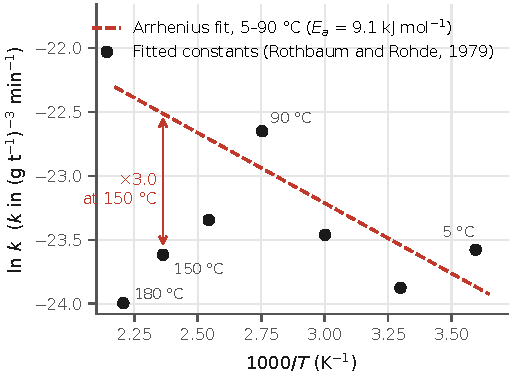
\includegraphics[width=.62\linewidth]{fig_paper_arrhenius}
\caption{Non-Arrhenius rate constant of amorphous-silica
polymerization. Fitted fourth-order rate constants $k(T)$ between 5 and
180~$^{\circ}$C from the primary data of \citet{rothbaum1979rohde}. The
dashed Arrhenius fit to the 5--90~$^{\circ}$C constants
($E_a = 9.1$~kJ/mol) overpredicts $k$ at 150~$^{\circ}$C by a factor of
3.0.}\label{fig:arrhenius}
\end{figure}

\begin{figure}[t]\centering
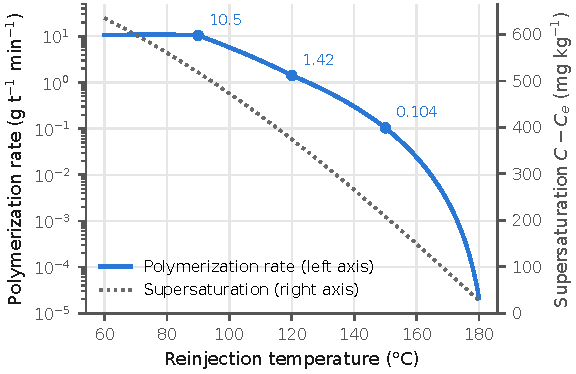
\includegraphics[width=.62\linewidth]{fig_paper_lever}
\caption{The reinjection-temperature lever. Uninhibited polymerization
rate (left axis) and supersaturation (right axis) versus reinjection
temperature for the archetype brine: Tiwi endmember B, 638~mg/kg
reservoir silica~\citep{sugiaman2004geochemical}, at a flash fraction of
0.25 (scenario input), giving 851~mg/kg in the separated brine;
solubility from \citet{gunnarsson2000amorphous}; kinetics from the
checksum-validated transcription of \citet{rothbaum1979rohde}. Cooling
from 150 to 90~$^{\circ}$C raises the rate by a factor of
101.}\label{fig:lever}
\end{figure}

\subsection{Test against independent laboratory data}\label{sec:labtest}

The kinetic core and the solubility correlation were tested against
data to which neither was fitted: the supplementary dataset of
\citet{scott2024silica}, read with the corrected parameterization of
\citet{scott2024corrigendum}. It comprises 61 monomeric-silica decay
experiments with 1{,}275 points spanning 23--80~$^{\circ}$C, pH
2.1--10.0 and ionic strength 0.01--0.53~mol/kg. Because the source is
machine-readable, transcription gives way to automated integrity
checks: unit headers are pinned, concentrations must decay
monotonically, replicate runs listed under duplicated identifiers are
separated, and one experiment in the colloid regime, outside the
dissolved-monomer scope, is flagged.

Two properties of the kinetic core are tested separately because they
fail differently. The first is the functional form. Linearizing the
integrated $n$-th-order decay law for $n = 2, \dots, 6$ in each
experiment shows that the decay of a single curve is second order in
supersaturation: the median $R^2$ is \NUM{KvRtwo} at $n = 2$ and
\NUM{KvRfour} at $n = 4$, falls steadily as the assumed order rises, and
order 2 fits best in all \NUM{KrN} qualifying near-neutral experiments
(pH 5--8; Fig.~\ref{fig:kinval}). This does
not contradict the classical law, which correlates the maximum rate
against the initial supersaturation across separate batches; the
integrated decay of one curve follows second-order kinetics of the
Rimstidt--Barnes type~\citep{rimstidt1980kinetics}. The two describe
different observables. The second property is the rate level. The
observed second-order constants follow an Arrhenius trend with
$E_a \approx$~\NUM{KvEa}~kJ/mol, and the ratio of the observed decay constant to
the one implied by the fitted core has a median of \NUM{KrMed}, ranging
from \NUM{KrMin} to \NUM{KrMax} across the \NUM{KrN} experiments: the
modern data decay six times faster than the classical law predicts at
the median. The median sets the fast-kinetics regime of
Section~\ref{sec:design}, and the spread shows that no fixed correction
of the transcribed law would reproduce the modern data.

The plateau of a nearly complete decay experiment is an independent
measurement of amorphous-silica solubility. Sixteen near-neutral
experiments that consumed at least 70\% of their initial
supersaturation level off at 0.90--1.37 times the
\citet{gunnarsson2000amorphous} correlation, with a median of 1.05. The
correlation and the 2024 endpoints therefore agree, and the band
$[0.90, 1.37]$ is the solubility range of the sensitivity study
(Section~\ref{sec:sobol}).

\begin{figure}[t]\centering
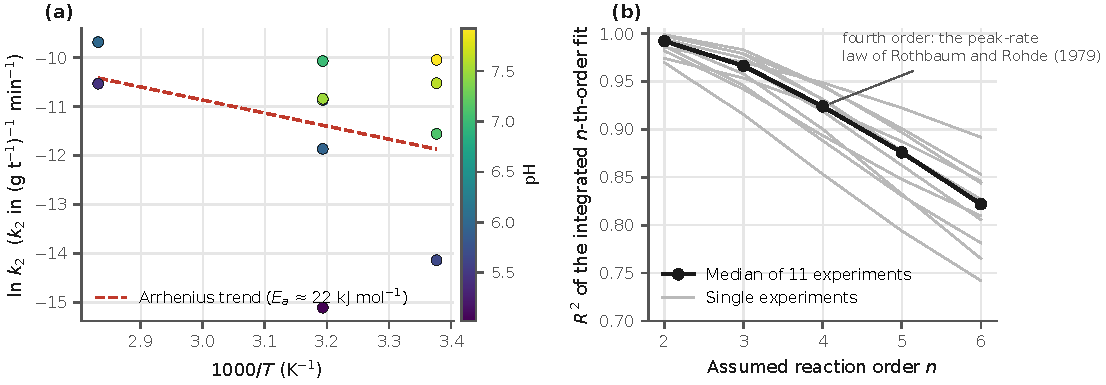
\includegraphics[width=\linewidth]{fig_paper_kinetics}
\caption{Test of the kinetic core against the independent data of
\citet{scott2024silica}. (a) Observed second-order rate constants of the
\NUM{KrN} near-neutral experiments (pH 5--8) versus inverse temperature,
coloured by pH, with the Arrhenius trend. (b) $R^2$ of the integrated
$n$-th-order linearization in each experiment (grey) and the median
(black): single-curve decay is second order, while the fourth-order
form of the classical law is a peak-rate law. Source:
\texttt{results/kinetics\_validation.csv}; panel (b) recomputed within
the same fitting window.}
\label{fig:kinval}
\end{figure}
